\RequirePackage[l2tabu, orthodox]{nag}
\documentclass[12pt]{article}

\usepackage[dvipsnames]{xcolor}
\usepackage{amssymb,amsmath,verbatim,graphicx,microtype,upquote,units,booktabs,hyperref,tikz,wrapfig,pgfplots,listings,tikz}
\usepackage[binary-units=true]{siunitx}
\usepackage[margin=10pt, font=small, labelfont=bf, labelsep=endash]{caption}
\usepackage[os=mac, mackeys=symbols]{menukeys}

\pgfplotsset{compat=1.12}
\setcounter{secnumdepth}{2}

\title{Project \#3}
\date{Due Date: Tuesday, December 6\textsuperscript{th}, 2016}
\author{Michael Schoen, Abdirahman Osman, Illya Starikov}

\newcommand{\shellcmd}[1]{\texttt{\colorbox{gray!30}{#1}}}
\newcommand{\todo}[1]{\textbf{\colorbox{red!50}{#1}}}
\newcommand{\br}{\\\multicolumn{2}{c}{} \\ }

\lstdefinestyle{cC}{
    language=C,
    basicstyle=\footnotesize\ttfamily,
    keywordstyle=\color{blue}\ttfamily,
    stringstyle=\color{red}\ttfamily,
    commentstyle=\color{gray}\ttfamily,
    morecomment=[l][\color{magenta}]{\#},
    numbers=left,
    keepspaces=true,
    tabsize=4,
    breaklines=true,
    morekeywords={true, false, bool}
}

\definecolor{amber}{rgb}{1.0, 0.75, 0.0}

\begin{document}
\maketitle

For the second project, we were delighted to be able to use a higher level programming language; we\footnote{Illya.} decided to apply this new-found excitement to implement a retro game from the \num{70}s: Space Invaders.

\begin{figure}[!ht]
    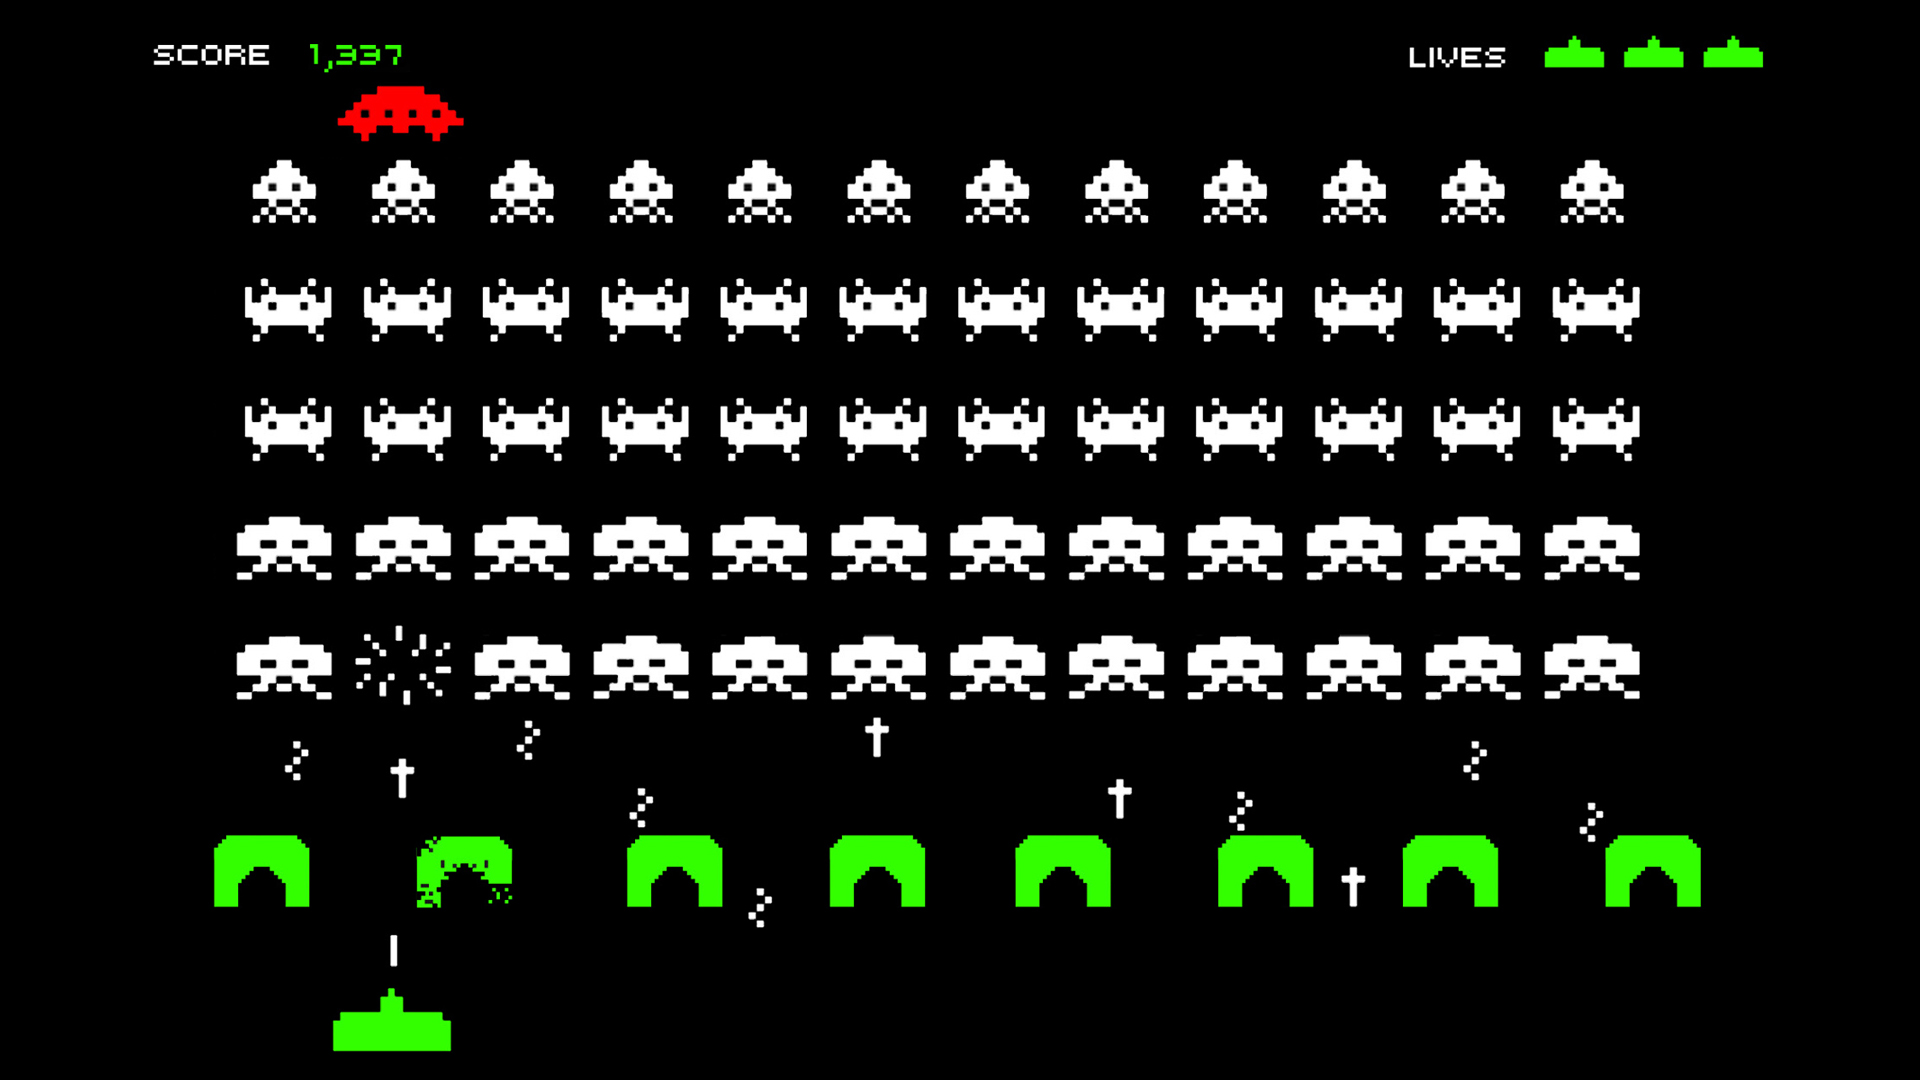
\includegraphics[width=\textwidth]{assets/space-invaders.jpg}
    \caption{The original space invaders.}
    \label{space-invaders}
\end{figure}

When this idea came crashing and burning down to the ground, we decided to combat this with a additional music, an elegant user interface, and a keyboard (with some other miscellanies).

\section{Project Description}
Below we will go into more detail about each individual parts of our project.

\subsection{The Game}
The game we initially decided to go with was space invaders. We had intention of doing the game logic on the microcontroller through serial communication; however, we learned early that this was likely not be possible\footnote{Our hex file with very basic functionality was \SI{25}{\kilo\byte}.}. We describe in \textit{Problems Encountered} how we absolved this. From here, we decided our game would exclusively be in the terminal.

Our game essentially creates a two dimensional array (in three segments --- the header to show score and level, the aliens, and the shooter). Then we loop through depending on the input:

\begin{description}
    \item[\keys{\arrowkeyleft}] Move the shooter left.
    \item[\keys{\arrowkeyright}] Move the shooter left.
    \item[\keys{q}] Quits the game
    \item[\keys{\SPACE}] Shoots with the gunner.
    \item[\keys{ }] No input meant refresh game.
\end{description}

We achieved the drawing through \shellcmd{curses}\footnote{Can be read about here \url{https://en.wikipedia.org/wiki/Curses_(programming_library)}}. Ultimately, we did not get our game fully done, but a good majority of it. See Figure. \ref{game} for a look at the UI of the game.

\begin{figure}[!ht]
    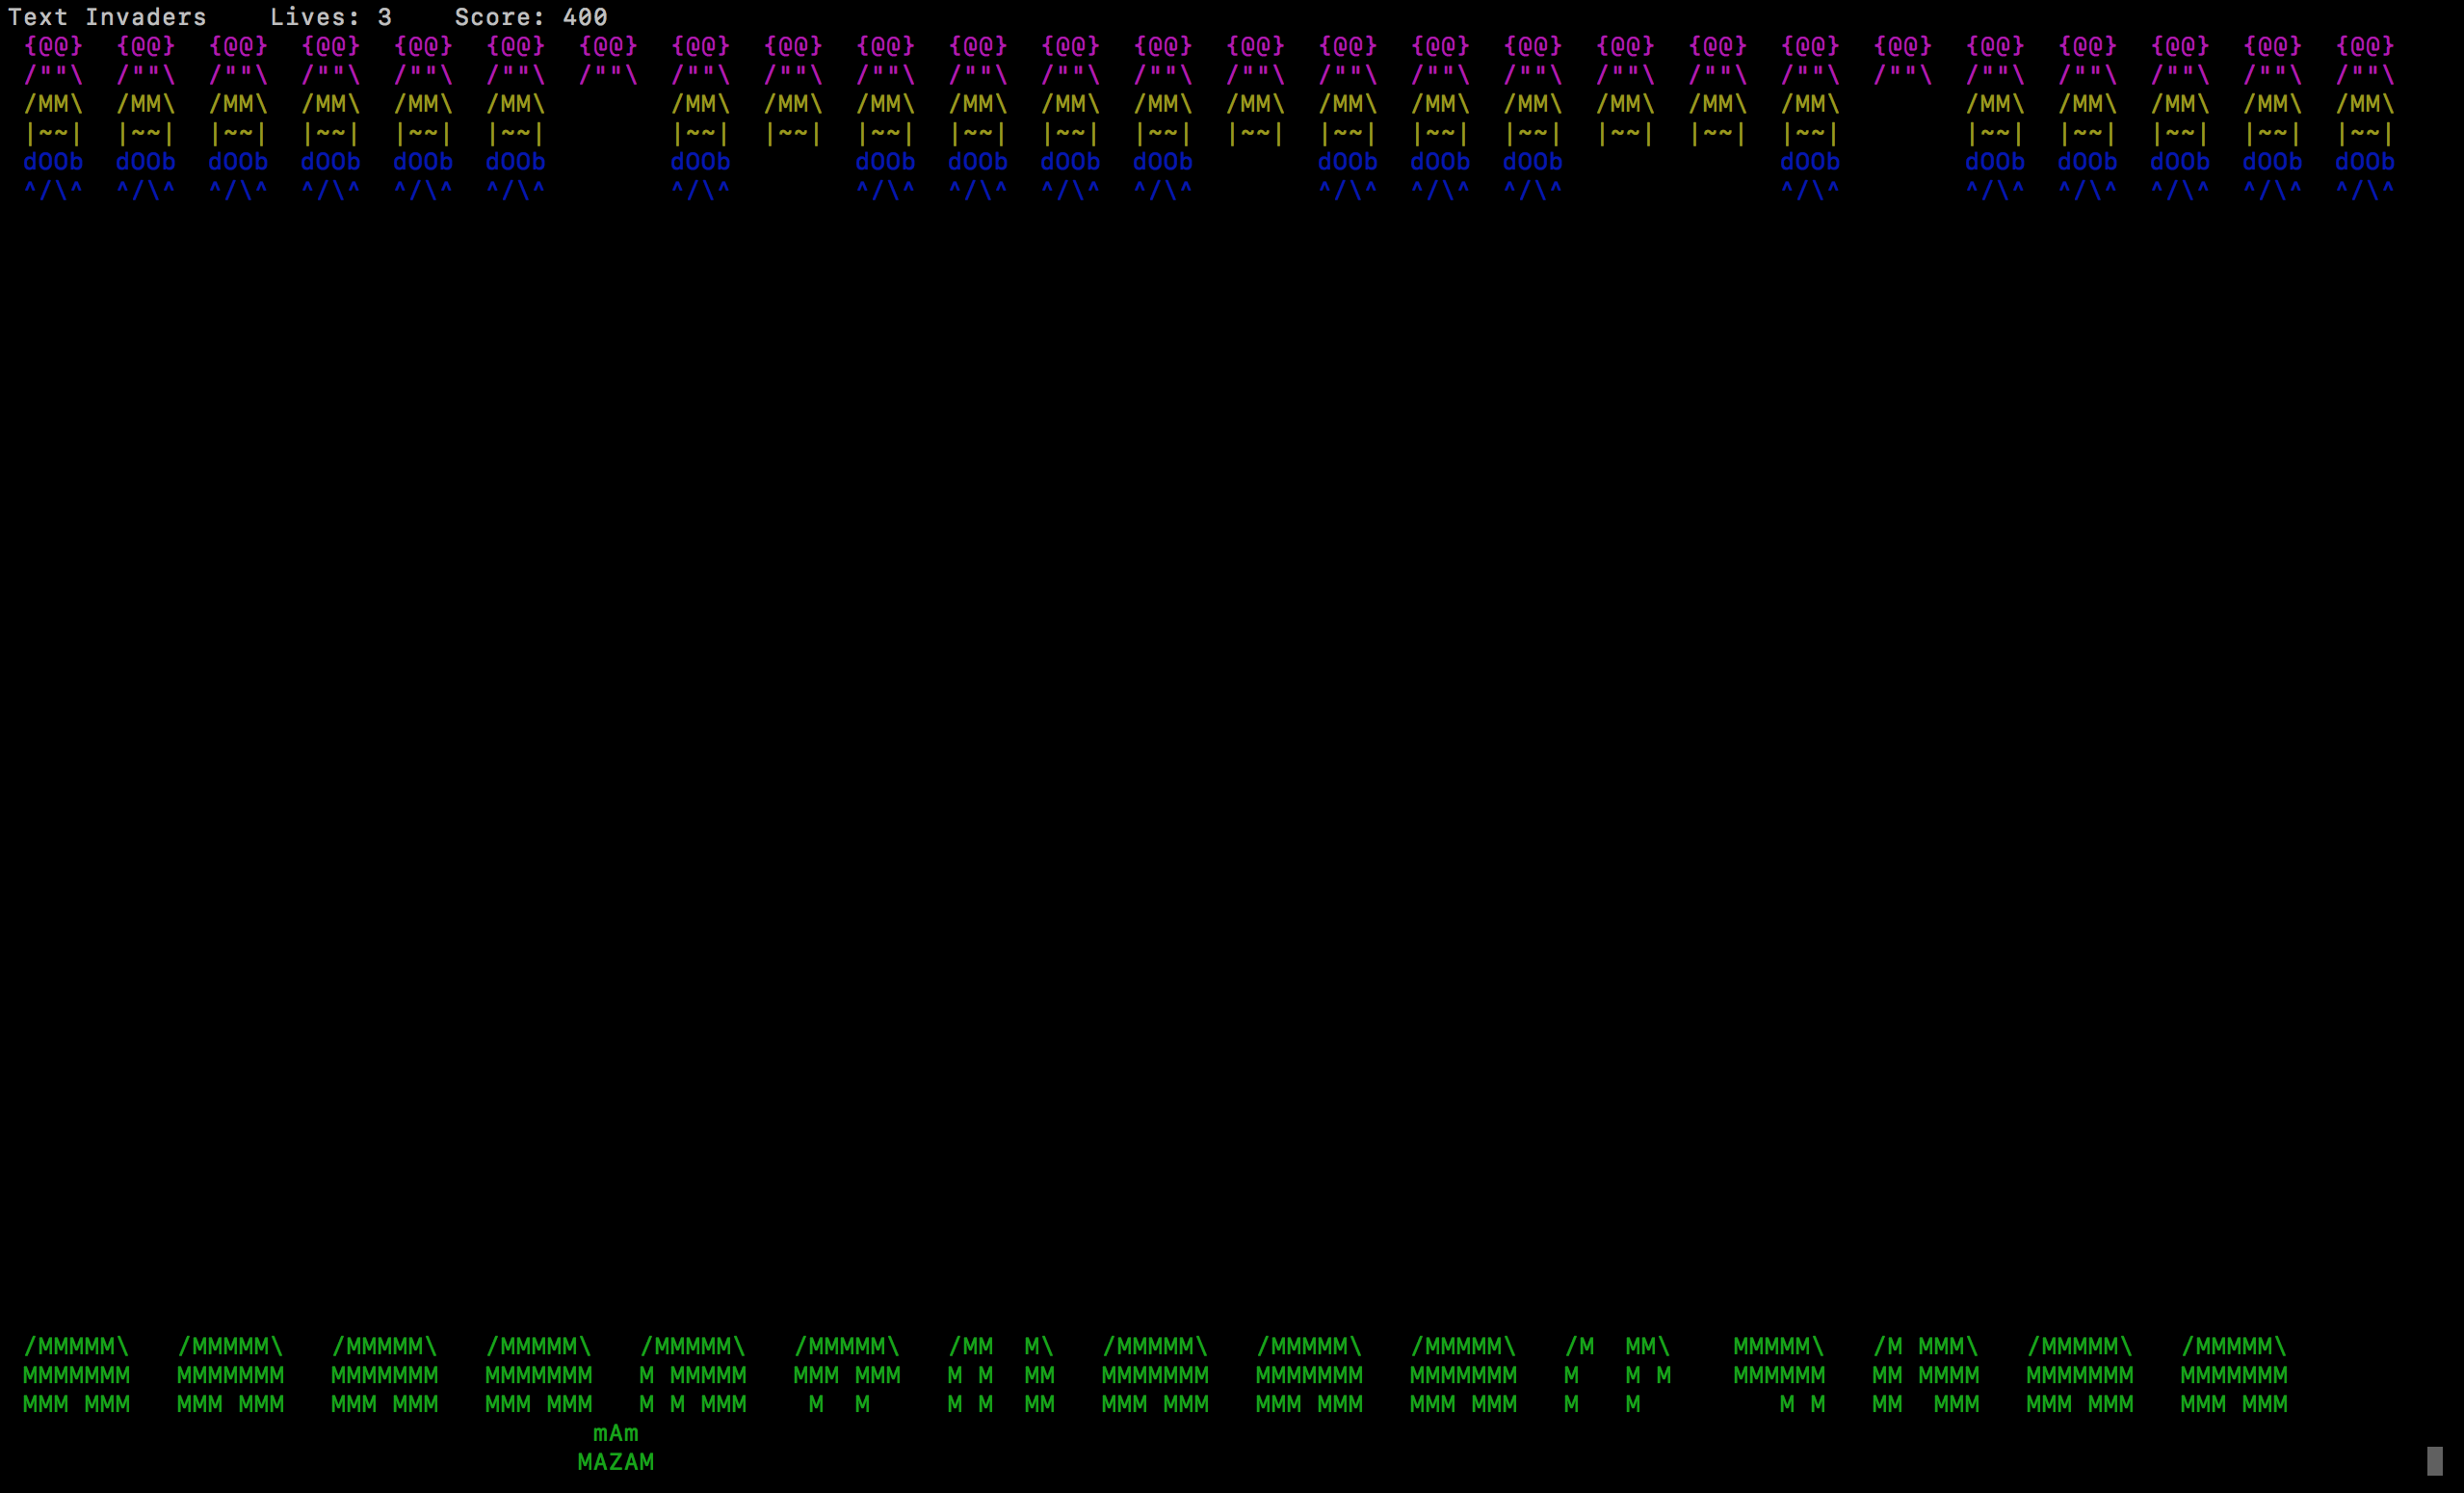
\includegraphics[width=\textwidth]{assets/game.png}
    \caption{Text Invaders, our version of space invaders..}
    \label{game}
\end{figure}

\subsection{Music}
The formula for each note is $$\frac{\nicefrac{1}{4} \, \text{Oscillator Frequency}}{\text{Note Frequency}}$$ So for supposing we want to produce the note $C4$,

\begin{equation}
    \frac{\nicefrac{1}{4} \, \text{Oscillator Frequency}}{\text{Note Frequency}} =
    \frac{\nicefrac{1}{4} \cdot \SI{7.373}{\hertz}}{\SI{261.63}{\hertz}} =
    \SI{7.045}{\milli\second}
\end{equation}

To produce the music, we had a function that took in which note and the type of note (\num{16}\textsuperscript{th}, \num{8}\textsuperscript{th}, \num{4}\textsuperscript{th}, half or whole note). The function multiplied the base length of a note by a constant depending on the type of note. A \num{16}\textsuperscript{th} note would be multiplied by \num{1}, an \num{8}\textsuperscript{th} by \num{2}, a quarter note by \num{4}, a half-note by \num{8}, and a whole note by \num{16}. We used timers and interrupts for the period of the note and the length of the note.

We also used sheet music to get the notes. For speeding and slowing down the music, the type of note was just multiplied by \num{2} or divided by \num{2} respectively.

\subsection{Interactive User Interface}
The menu goes through three stages; printing the pen-rose triangle background, printing options, then allowing the selection of items. The following are printed

\begin{enumerate}
    \item Counter
    \item Hurricane's Eye
    \item Keyboard
\end{enumerate}

\noindent respectively. From there the user has the option to to cycle upwards using $P_2$ (see Figure. \ref{menu}), cycle down using $P_8$, or select using $P_5$. The cycle starts with \num{1}, highlighting Counter if $P_2$ is pressed, then Hurricane's eye will be highlighted, and if printed once again Counter will be selected. If the menu user presses $P_1$ once at the 3rd option (Keyboard) then the menu will cycle back to option \num{1} and vice versa if $P_8$ were clicked at the 1st option. Selecting an menu option with $P_5$ while highlighted will start its respective function. Also each menu option has a corresponding number displayed on a seven segment display.

\begin{figure}[!ht]
    \centering
    \begin{tikzpicture}
        \node[draw,circle,minimum size=1cm,fill=red,inner sep=0pt] (1) at (0,4) {$P_1$};
        \node[draw,circle,minimum size=1cm,fill=yellow,inner sep=0pt] (2) at (2,4) {$P_2$};
        \node[draw,circle,minimum size=1cm,fill=green,inner sep=0pt] (3) at (4,4) {$P_3$};

        \node[draw,circle,minimum size=1cm,fill=amber,inner sep=0pt] (4) at (0,2) {$P_4$};
        \node[draw,circle,minimum size=1cm,fill=blue,inner sep=0pt] (5) at (2,2) {$P_5$};
        \node[draw,circle,minimum size=1cm,fill=red,inner sep=0pt] (6) at (4,2) {$P_6$};

        \node[draw,circle,minimum size=1cm,fill=yellow,inner sep=0pt] (7) at (0,0) {$P_7$};
        \node[draw,circle,minimum size=1cm,fill=green,inner sep=0pt] (8) at (2,0) {$P_8$};
        \node[draw,circle,minimum size=1cm,fill=amber,inner sep=0pt] (9) at (4,0) {$P_9$};
    \end{tikzpicture}
    \caption{The Main Menu.}
    \label{menu}
\end{figure}

\subsection{Seven Segment Display}
For the seven segment display, we had to set $P_2$ to be push/pull so that the display would receive enough power. We then looked up the correct values to output to the pins to make each number show up on the display and used those values in the increment/decremented function as well as the simple function that lets you display any number. We used the data sheet for the seven segment display to see how to connect it on the breadboard. See Figure. \ref{schematic} for additional information.

\begin{figure}[!ht]
    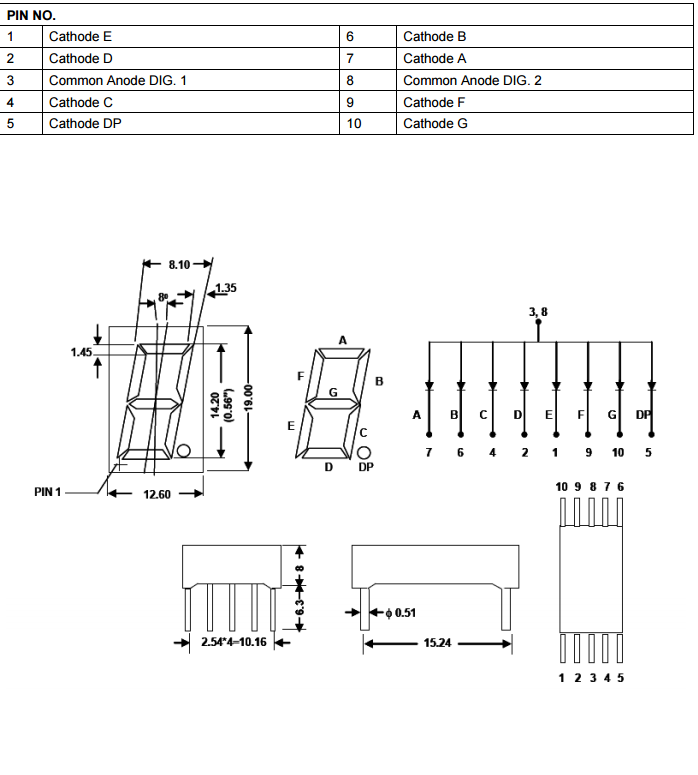
\includegraphics[width=\textwidth]{assets/scematic}
    \caption{The schematic for the seven segment display.}
    \label{schematic}
\end{figure}

\subsection{Keyboard}
Our keyboard has a C scale set to switches $P_1 \cdots P_8$ with $P_9$ escaping to the menu. Each switch uses the corresponding light associated with its position save $P_9$ which is the escape button.

\subsection{Curses}
In order to print to any part of the screen we needed to implement a structure to send ANSI control sequences and characters to the terminal using \shellcmd{uart\_get()} as a base. To do this we implemented an \num{8051} port of curses that takes in $(x,\, y)$ coordinates as arguments for printing \shellcmd{chars} and \shellcmd{strings} at any defined $(x,\, y)$ location. This allows for the implementation of the menu since it requires printing of options in sometimes nonlinear fashion.

We found a whole host of others issues associated with printing characters to a terminal, printing to an arbitrary location, control sequences, fluctuation in crystal timings, and requesting information from a terminal. We accounted for these individually.

\section{Problems Encountered}
Below we will list some of the ``several'' problems we ran into.

\subsection{Memory Constraints}
By far, the biggest problem we encountered was the memory constraint. The \SI{8051} has \SI{8}{\kilo\byte} of memory; our code base, with the exclusion of all the \shellcmd{malloc}s\footnote{Since \shellcmd{unsigned char} = \SI{1}{\byte}, the terminal window will roughly be $20\text{ height} \times 80\text{ width} $, we can roughly expect \SI{1.6}{\kilo\byte} to be allocated on the heap; a non-insignificant amount compared to \SI{8}{\kilo\byte}.}, it is roughly \SI{25}{\kilo\byte} --- a size a bit larger than the \num{8051} allows. Our workaround was to fight fire with fire.

Instead of ``dumbing'' down our game\footnote{According to back of the hand calculations, a space-optimized version of the game would still be \SI{7}{\kilo\byte}. This was likely to be impossible.} to get it to fit, we decided to have an external interface; specifically, a port sniffer. It would listen for input from the \num{8051}, and if there is a signal on the serial port, use that as input. If not, default to the keyboard input.

Ultimately, we were unsuccessful with the port sniffer. Originally, we had tried to use a Linux port sniffer so we can just embed it into our program, \shellcmd{slsnif}\footnote{Can be found at \url{https://sourceforge.net/projects/slsnif/}.}. Unfortunately this port sniffer does not support ``legacy'' ports, and the \num{8051} falls in this category. So we moved onto a Windows port sniffer, \shellcmd{Serial Input For Windows}\footnote{Can be found at \url{http://www.randomnoun.com/wp/2013/02/03/serial-input-for-windows/}.}. This too did not work, because we could only have one interface use the serial port, so we would need a dedicated socket to intercept the \shellcmd{COM1} port's input --- something we were not familiar with.

Ultimately, we were simply unsuccessful and had to scrap this.

\subsection{Printing Lines and Columns.}
We had an issue with the timing crystals of the Simon board where the board heating up would cause the serial port to start printing unrecognizable characters. This lead us to think we were causing a segfault when we was printing string literals. This caused hours of wasted time since nothing we could change would cause the board to start printing what we wanted, but one afternoon after hours of exhaustive research and help at the lead sessions the conclusion was reached that heat changes were causing the board to lose its timing and print out nonsense. The fix for this was to let the board cool off while writing code. After this change garbage outputs dropped significantly.

\subsection{Seven Segment Display Buttons}
One problem we ran into was some of the buttons use the same pins as we used for the seven segment display. The display used push/pull which makes the buttons not work, so we had to carefully chose buttons that didn't use the same pins.

\section{8051 Architecture}
For this project, we made sure to utilize the additional functionality we learned in the later parts of the semester --- specifically, timers, serialization, and interrupts.

We spent a great deal of time with the serial communication aspect of the board; we took advantage of this the most (with respect to the \num{8051} architecture). We have already discussed the things that made our board unique; however, we will show an example of how our implimination of \shellcmd{curses}.

\begin{lstlisting}[style=cC]
void move(unsigned char y, unsigned char x) {
	unsigned char i; // counter
	zero_cursor(); // moves the code to (0, 0)

	for(i = 0; i < x; i++) {
		cursor_jump(1, 'R'); // move cursor to the x position
	}
	for(i=0; i < y; i++) {
		cursor_jump(1, 'D'); // now to the y
	}
}
\end{lstlisting}

\noindent Now combining that with \shellcmd{addch(char)},

\begin{lstlisting}[style=cC]
void addch(unsigned char value) {
	uart_isr();
	uart_transmit(value);
	while(TI==0);
}
\end{lstlisting}

\noindent we have a fundamental a functionality to \shellcmd{curses}, printing anywhere!

Next, we implemented all delays with timer interrupts. For example,

\begin{lstlisting}[style=cC]

void delay1ms() {
	TH0=-0x0E;
    TL0=-0x66;
	TR0 = 1; // start
	while(TF0 == 0); // poll to finish
	TR0 = 0; // stop
	TF0 = 0; // clear the finish
}
\end{lstlisting}

\noindent delays for \SI{1}{\milli\second}, because $(\text{FFFF}_{16} - \text{0E66}_{16} + 1)\times\SI{1.085}{\micro\second} \approx \SI{1}{\milli\second}$. As it turns out, we mostly needed millisecond precision, so we used this as the foundation for the rest of the program.

\section{Individual Features}
\begin{itemize}
    \item Michael Schoen --- 33\% Contribution
    \begin{itemize}
        \item Song
        \item Seven Segment Display
    \end{itemize}

    \item Abdirahman Osman --- 33\% Contribution
    \begin{itemize}
        \item Port Serialization
        \item Text User Interface
        \item Menu
    \end{itemize}

    \item Illya Starikov --- 33\% Contribution
    \begin{itemize}
        \item Space Invaders Game
        \item Keyboard
    \end{itemize}
\end{itemize}

\centering
\Huge Happy Holidays \\ From Michael, Abdirahman, and Illya!

\end{document}
